\documentclass{X:/Documents/Coding/Latex/myassignment}
%%Document info
\title{OFN Assignment 4}
\begin{document}
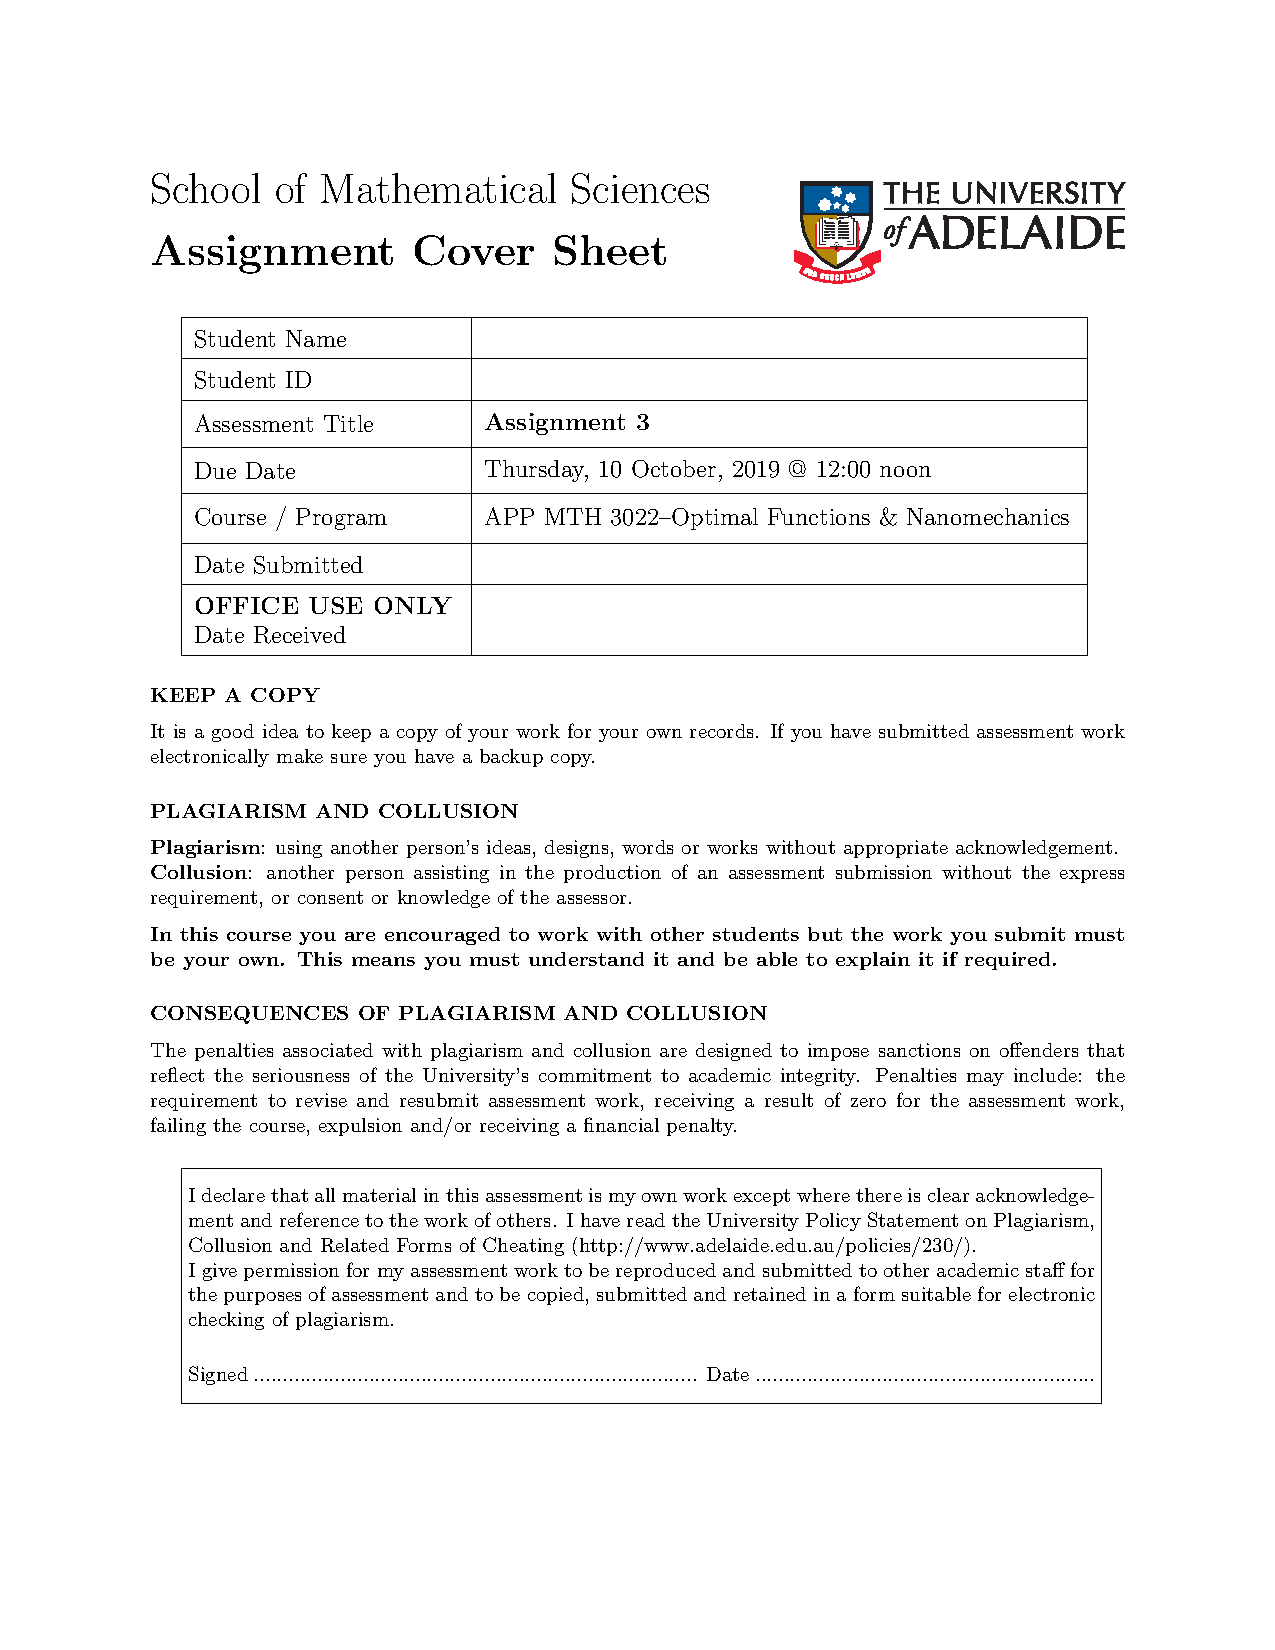
\includepdf{cover4}
\maketitle

\begin{enumerate}
%1
\item 
\begin{enumerate}
	%1a
	\item $dA$ is obtained using the cross product of the tangent vectors of the parametrisation
	\begin{align*}
		\dd r\theta &= \left(-b\sin\theta \sin\phi, b\cos\theta\sin\phi,0\right)\\
		\dd r\phi &= \left(b\cos\theta\cos\phi, b\sin\theta\cos\phi,-c\sin\phi\right)
	\end{align*}

	\[dA = \left|\dd r\theta \times \dd r\phi \right| d\theta d\phi\]
	\[\dd r\theta \times \dd r\phi= \begin{vmatrix}
		\vec i & \vec j & \vec k \\
		-b\sin\theta \sin\phi& b\cos\theta\sin\phi&0\\
		b\cos\theta\cos\phi& b\sin\theta\cos\phi&-c\sin\phi
	\end{vmatrix}\]
	\begin{align*}
		\dd r\theta \times \dd r\phi&= \left(-bc\cos\theta\sin^2\phi, -bc\sin\theta\sin^2\phi, -b^2\sin^2\theta\sin\phi\cos\phi - b^2\cos\theta^2\sin\phi\cos\phi\right)\\
		&=\left(-bc\cos\theta\sin^2\phi, -bc\sin\theta\sin^2\phi, -b^2\sin\phi\cos\phi\right) \\
		&= b\sin\phi \det \left(-c\cos\theta\sin\phi, -c\sin\theta\sin\phi, -b\cos\phi\right) \\
	\end{align*}
	\begin{align*}
	dA &= \left|\dd r\theta \times \dd r\phi \right| d\theta d\phi\\
		&= b\sin\phi\sqrt{(-c\cos\theta\sin\phi)^2 + (-c\sin\theta\sin\phi)^2 + (-b\cos\phi)^2} d\theta d\phi\\
		&= b\sin\phi\sqrt{c^2\cos^2\theta\sin^2\phi + c^2\sin^2\theta\sin^2\phi + b^2\cos^2\phi} d\theta d\phi\\
		&= b\sin\phi\sqrt{c^2\sin^2\phi + b^2\cos^2\phi} d\theta d\phi\\
		&= b\sin\phi\sqrt{c^2\sin^2\phi + b^2(1-\sin^2\phi)} d\theta d\phi\\
		&= b\sin\phi\sqrt{(c^2-b^2)\sin^2\phi + b^2} d\theta d\phi\\
	\end{align*}
	% 1b
	\item The surface area:
	\begin{align*}
		A &= \int_{0}^{\pi}\int_{-\pi}^{\pi} b\sin\phi\sqrt{(c^2-b^2)\sin^2\phi + b^2}d\theta d\phi\\
		&= 2\pi b  \int_{0}^{\pi} \sin\phi\sqrt{(c^2-b^2)\sin^2\phi + b^2} \ d\phi\\
		&= 2\pi b \left( \int_{0}^{\pi/2} \sin\phi\sqrt{(c^2-b^2)\sin^2\phi + b^2} \ d\phi +  \int_{\pi/2}^{\pi} \sin\phi\sqrt{(c^2-b^2)\sin^2\phi + b^2} \ d\phi\right)\\
		&= 2\pi b \left( \int_{0}^{\pi/2} \sin\phi\sqrt{(c^2-b^2)\sin^2\phi + b^2} \ d\phi \right.\\&\qquad+\left.  \int_{0}^{\pi/2} \sin(\phi+\pi/2)\sqrt{(c^2-b^2)\sin^2(\phi+\pi/2) + b^2} \ d\phi\right)\\
		&= 2\pi b \left( \int_{0}^{\pi/2} \sin\phi\sqrt{(c^2-b^2)\sin^2\phi + b^2} + \cos\phi\sqrt{(c^2-b^2)\cos^2\phi + b^2} \ d\phi\right)\\
	\end{align*}
	% Let $t = \sin\phi$, $d\phi  = \cos\phi dt = \sqrt{1-t^2} dt$
	Let $t = \sin^2\phi$, $d\phi = 2\cos\phi\sin\phi dt = 2\sqrt{t}\sqrt{1-t} d\theta$
% \begin{align*}
% 		A &= 2\pi b \left( \int_{0}^{\pi/2} \sin\phi\sqrt{(c^2-b^2)\sin^2\phi + b^2} + \cos\phi\sqrt{(c^2-b^2)\cos^2\phi + b^2} \ d\phi\right)\\
% 		&= 2\pi b \left( \int_{0}^{1} 2\sqrt{t}\sqrt{t}\sqrt{1-t}\sqrt{(c^2-b^2)t + b^2} + 2\sqrt{t}\sqrt{1-t}^2\sqrt{(c^2-b^2)(1-t) + b^2} \ dt\right)\\
% 		&= 4\pi b \left( \int_{0}^{1} t\sqrt{1-t}\sqrt{(c^2-b^2)t + b^2} + \sqrt{t}(1-t)\sqrt{(c^2-b^2)(1-t) + b^2} \ dt\right)\\
% 		&= 4\pi b \left( \int_{0}^{1} bt\sqrt{1-t}\sqrt{1 - (1-\frac{c^2}{b^2})t} + b\sqrt{t}(1-t)\sqrt{(\frac{c^2}{b^2}-1)(1-t) + 1} \ dt\right)\\
% 		&= 4\pi b \left( \int_{0}^{1} bt\sqrt{1-t}\sqrt{1 - (1-\frac{c^2}{b^2})t} + b\sqrt{t}(1-t)\sqrt{\frac{c^2}{b^2} - t \frac{c^2}{b^2}  - t} \ dt\right)\\
% 		&= 4\pi b \left(b \int_{0}^{1} t\sqrt{1-t}\sqrt{1 - (1-\frac{c^2}{b^2})t} dt + c\int_0^1 \sqrt{t}(1-t)\sqrt{1 - (\frac{b^2}{c^2} + 1)t} \ dt\right)\\
% \end{align*}
\begin{align*}
		A &= 2\pi b \left( \int_{0}^{\pi/2} \sin\phi\sqrt{(c^2-b^2)\sin^2\phi + b^2} + \cos\phi\sqrt{(c^2-b^2)\cos^2\phi + b^2} \ d\phi\right)\\
		&= 2\pi b \left( \int_{0}^{1} \frac{1}{2\sqrt{t}\sqrt{1-t}}\sqrt{t}\sqrt{(c^2-b^2)t + b^2} +  \frac{1}{2\sqrt{t}\sqrt{1-t}}\sqrt{1-t}\sqrt{(c^2-b^2)(1-t) + b^2} \ dt\right)\\
		&= \pi b \left( \int_{0}^{1} \frac{1}{\sqrt{1-t}}\sqrt{(c^2-b^2)t + b^2} +  \frac{1}{\sqrt{t}}\sqrt{(c^2-b^2)(1-t) + b^2} \ dt\right)\\
		&= \pi b \left( b\int_{0}^{1} \frac{1}{\sqrt{1-t}}\sqrt{1 + (\frac{c^2}{b^2}-1)t} +  \frac{c}{\sqrt{t}}\sqrt{(1-\frac{b^2}{c^2})(1-t) + \frac{b^2}{c^2}} \ dt\right)\\
		&= \pi b \left( b\int_{0}^{1} \frac{1}{\sqrt{1-t}}\sqrt{1 + (\frac{c^2}{b^2}-1)t} +  \frac{c}{\sqrt{t}}\sqrt{1 - (1-\frac{b^2}{c^2})t}\ dt\right)\\
		&= \pi b \left( b\int_{0}^{1} \frac{1}{\sqrt{1-t}}\sqrt{1 - (1-\frac{c^2}{b^2})t}dt +  c \int_0^1\frac{1}{\sqrt{t}}\sqrt{1 - (1-\frac{b^2}{c^2})t} \ dt\right)\\
\end{align*}
	The Euler form of the hypergeometric function is:
	\[F(a,b;c;z) = \frac{\Gamma(c)}{\Gamma(b)\Gamma(c-b)}\int_0^1 x^{b-1} (1-x)^{c-b-1} (1- zx)^{-a} dx\]

	The first integral is hypergeometric with 
	\[a_f = -1/2,\quad  b_f = 1,\quad  c_f = 3/2, \quad \text{and} \quad z_f = 1-\frac{c^2}{b^2}\]
	And the second with
	\[a_{f2} = -1/2,\quad b_{f2} = 1/2,\quad  c_{f2} = 3/2, \quad \text{and} \quad z_{f2} = 1 -\frac{b^2}{c^2}\]
	Hence it can be written as
	\begin{align*}
		A &= 4\pi b \left(b \frac{\Gamma(1) \Gamma(1/2)}{\Gamma(3/2)} F\left(-1/2,1,3/2,1- \frac{c^2}{b^2}\right) + c\frac{\Gamma(1/2) \Gamma(1)}{\Gamma(3/2)} F\left(-1/2,1/2,3/2, 1- \frac{b^2}{c^2}\right) \right)\\
		&= \pi b \frac{\sqrt{\pi} }{\sqrt{\pi}/2} \left(bF\left(-1/2,1,3/2,1- \frac{c^2}{b^2}\right) + cF\left(-1/2,1/2,3/2,1 - \frac{b^2}{c^2}\right)  \right)\\
		A&= 2\pi b \left(bF\left(-1/2,1,3/2,1- \frac{c^2}{b^2}\right) + cF\left(-1/2,1/2,3/2,1 -\frac{b^2}{c^2}\right)  \right)\\
	\end{align*}

	% 1c
	\item Mean atomic surface density is the number of atoms divided by the surface area of the molecule. For a $C_{70}$ fullerene the surface density is given by
	\begin{align*}
		\eta &= \frac{70}{A}\\
	\end{align*}
 	This is solved numerically in the code, giving:
 	\begin{lstlisting}
eta =

     0.1948
 	\end{lstlisting}
\end{enumerate}

%question 2
\item Minimising the surface area of the soap film.
\begin{enumerate}
	%2a
	\item Parameterise the position on the surface as
	\[\vec r = \left(r(z)\cos u, r(z)\sin u, z\right)\]
	\begin{align*}
		\dd{\vec r}{u} &= \left(-r\sin u, r \cos u, 0\right)\\
		\dd{\vec r}{z} &= \left(r'\cos u, r'\sin u,1\right)\\
		\dd{\vec r}{u} \times \dd{\vec r}{z} &= \left(r\cos u, r\sin u, -rr' \sin^2 u - rr' \cos^2 u\right)\\
		&=r(\cos u, \sin u, -r')
	\end{align*}
	The delta surface area:
	\begin{align*}
		dA &= \left|\dd{\vec r}{u} \times \dd{\vec r}{z}\right| du dz\\
		&= r\sqrt{\cos^2 u + \sin^2 u + r'^2} du dz\\
		&= r \sqrt{1 + r'^2} du dz
	\end{align*}
	So the surface area, for $r_0 = 9$ and $r_1 = 10$, is: 
	\begin{align*}
		S &= \int_{z_0}^{z_1} \int_{-\pi}^{\pi}  r \sqrt{1 + r'^2} du dz\\
		&= 2\pi \int_{z_0}^{z_1}  r \sqrt{1 + r'^2} dz\\
		\implies S &= 2\pi \int_{z_0}^{z_1} r\sqrt{1 + r'^2} dz = \int_{z_0}^{z_1} s(r,r') dz\\
	\end{align*}
	We want to minimise $S$, and so the E-L equation is (since it doesn't explicitly contain z):
	\begin{align*}
		\dd{s}{r} &- \odd{}z \left(\dd s{r'}\right) = 0\\
		H &=r' \dd{s}{r'} - s = c\\
	\end{align*}
	\begin{align*}
	r'\frac{r r'}{\sqrt{1+r'^2}} - r\sqrt{1 + r'^2} & = c\\
	r r'^2 - r - r r'^2 &= c\sqrt{1 + r'^2}\\	
	-r &= c\sqrt{1+r'^2}\\
	r^2 &= c(1+r'^2)\\
	c^2 r'^2 &= r^2 - c^2\\
	r' &= \pm \frac{1}{c}\sqrt{r^2 - c^2}\\
	\end{align*}
	Separable DE:
	\begin{align*}
		\int\frac{1}{\sqrt{r^2 - c^2}}dr &= \pm \int \frac{1}{c} dz\\
		\int \frac{1}{\sqrt{u^2 - 1}} du &= \pm \int \frac{1}{c} dz,\quad \left( u = \frac{r}{c}\right)\\
	\end{align*}
	As in lectures, let $u = \cosh(v)$  and $du = \sinh(v) dv$
	\begin{align*}
		\int \frac{\sinh v}{\sqrt{\cosh^2v - 1}} du &= \pm \frac{1}{c}\int dz\\
		\int \frac{\sinh v}{\sqrt{\sinh^2v}} dv &= \pm \frac{1}{c}\int dz\\
		\int 1 dv &= \pm \frac{1}{c}\int dz\\
		v &= \pm \frac{z}{c} + b\\
		\mathrm{arcosh}(\frac{r}{c}) &= \pm \frac{z}{c} + b\\
		\frac{r}{c} &= \cosh\left(\pm \frac{z}{c} + b\right)\\
		r &= c\cosh\left(\pm \frac{z}{c} + b\right)\\
	\end{align*}
	Since $\cosh$ is even, and $b$ is an arbitrary constant, the $\pm$ can be ignored.
	\[r = c\cosh\left(\frac{z+b}{c}\right)\]
	BCs:
	\begin{align*}
		r(0) = 9 = c\cosh\left(\frac{b}{c}\right)\\
		r(1) = 10 = c\cosh\left(\frac{10 + b}{c}\right)\\
	\end{align*}
	Solving in matlab gives to 4sf:
	\[b = -4.272, \quad c = 7.801\]

	%2b
	\item Plotted in figure~\ref{fig:soap}. 

	\begin{figure}[tbh]
		\centering
		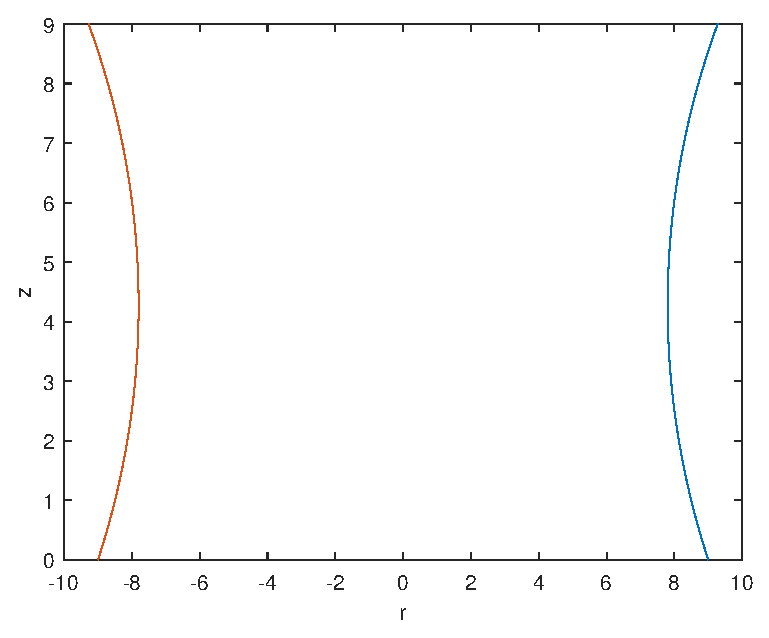
\includegraphics[width=0.8\linewidth]{A4Plot.eps}
		\caption{Profile of the soap film. Both the $r$ and $-r$ profiles are shown.}
		\label{fig:soap}
	\end{figure}
\end{enumerate}
%question 3
\item Extremal calculation using Ritz' method
	\begin{align*}
		\bar{y} &= c_1\phi_1(x) + c_2 \phi_2(x)\\
		&= c_1(1-x^2) + c_2(1-x^4)\\\\
		\bar{y}' &= c_1\phi_1'(x) + c_2 \phi_2'(x)\\
		&= c_1(-2x) + c_2(-4x^3)
	\end{align*}

	\begin{align*}
		\bar{y}^2 &= (c_1(1-x^2) + c_2(1-x^4))^2 \\
		&= c_1^2(1 - 2x^2 + x^4) + 2c_1c_2 (1-x^2)(1-x^4) + c_2^2 (1 - 2x^4 + x^8)\\
		&= c_1^2(1 - 2x^2 + x^4) + 2c_1c_2 (1 - x^2 -x^4 + x^6) + c_2^2 (1 - 2x^4 + x^8)\\
	\end{align*}
	\begin{align*}
		\bar{y}'^2 &= (c_1(-2x) + c_2(-4x^3))^2\\
		&= 4c_1^2x^2 +16c_1c_2 x^4+ 16c_2x^6
	\end{align*}

	\begin{align*}
		F\{\bar{y}\} &= \int_0^1 x(\bar{y}'^2 - \lambda \bar{y}^2) dx\\
		&= \int_0^1 x((-2c_1x - 4c_2x^3)^2 - \lambda (c_1(1-x^2) + c_2(1 - x^4)^2) dx\\
		&= \int_0^1 x((2c_1x + 4c_2x^3)^2 - \lambda (c_1^2(1-x^2)^2 + 2c_1c_2(1-x^2)(1-x^4) + c_2^2(1-x^4)^2 )) dx\\
		&= \int_0^1 x(4c_1^2x^2 + 16c_1c_2x^4 + 16c_2^2x^6 \\&- \lambda (c_1^2(1-2x^2 + x^4) +2c_1c_2 (1-x^2 - x^4 + x^6) +  c_2^2(1 - 2x^4 + x^8))) dx\\
		&= \int_0^1 4c_1^2x^3 + 16c_1c_2x^5 + 16c_2^2x^7 \\&- \lambda (c_1^2(x-2x^3 + x^5) +2c_1c_2 (1-x^3 - x^5 + x^7) +  c_2^2(x - 2x^5 + x^9)) dx\\
		&=\left[c_1^2x^4 + \frac{16}{6}c_1c_2x^6 + 2c_2^2x^8 \right.\\&\left.- \lambda (c_1^2(\frac{1}{2}x^2-\frac{1}{2}x^4 + \frac{1}{6}x^6) +2c_1c_2 (\frac{1}{2}x^2-\frac{1}{4}x^4 - \frac{1}{6}x^6 + \frac{1}{8}x^8) +  c_2^2(\frac{1}{2}x^2 - \frac{1}{3}x^6 + \frac{1}{10}x^{10}))\right]_0^1 \\\\
	\end{align*}
	\begin{align*}
	F\{\bar{y}\} &= c_1^2 + \frac{16}{6}c_1c_2 + 2c_2^2 %\\&
	- \lambda (c_1^2(\frac12-\frac{1}{2} + \frac{1}{6}) +2c_1c_2 (\frac{1}{2}-\frac{1}{4} - \frac{1}{6} + \frac{1}{8}) +  c_2^2(\frac{1}{2} - \frac{1}{3} + \frac{1}{10}))\\
		F &=  {c_{1}}^2+\frac{8 c_{1} c_{2}}{3}+2 {c_{2}}^2-\lambda\left(\frac{{c_{1}}^2 }{6}+\frac{5 c_{1} c_{2} }{12}+\frac{4 {c_{2}}^2 }{15}\right)\\
		&=  c_1^2 \left(1 - \frac{\lambda}{6}\right)  + c_1c_2 \left(\frac{8}{3} - \frac{5\lambda}{12}\right) + c_2^2\left(2 - \frac{4\lambda }{15}\right)
	\end{align*}

	\begin{align*}
		% \dd{F}{\lambda} &=  \frac{{c_{1}}^2 }{6}+\frac{5 c_{1} c_{2} }{12}+\frac{4 {c_{2}}^2 }{15} = 0\\
		\dd{F}{c_1} &=2c_1 \left(1 - \frac{\lambda}{6}\right) + c_2 \left(\frac{8}{3} - \frac{5\lambda}{12}\right) = 0\\
		\dd{F}{c_2} &=c_1\left(\frac{8}{3} - \frac{5\lambda}{12}\right) + 2c_2 \left(2 - \frac{4\lambda}{15}\right) = 0
	\end{align*}
	% \begin{align*}
	% 2c_1 \left(1 - \frac{\lambda}{6}\right) + c_2 \left(\frac{8}{3} - \frac{5\lambda}{12}\right) = 0\\
	% 	\lambda \left(2c_1 \frac{1}{6} + c_2 \frac{5}{12}\right) = 2c_1 + c_2 \left(\frac{8}{3} \right)\\
	% 	\lambda =\frac{2c_1 + \frac{8c_2}{3}}{ \frac{c_1}{3} + \frac{5c_2}{12}}
	% \end{align*}
	% \begin{align*}
	% 	c_1\left(\frac{8}{3} - \frac{5\lambda}{12}\right) + 2c_2 \left(2 - \frac{4\lambda}{15}\right) = 0\\
	% 	\lambda \left(\frac{5c_1}{12} + \frac{8c_2}{15}\right) = \frac{8c_1}{3} + 4c_2\\
	% 	\lambda = \frac{\frac{8c_1}{3} + 4c_2}{\frac{5c_1}{12} + \frac{8c_2}{15}}
	% \end{align*}

	% Both of these must be satisfied for non-trivial solutions. Hence

	% \begin{align*}
	% 	\frac{2c_1 + \frac{8c_2}{3}}{ \frac{c_1}{3} + \frac{5c_2}{12}} &= \frac{\frac{8c_1}{3} + 4c_2}{\frac{5c_1}{12} + \frac{8c_2}{15}}\\
	% 	\left(2c_1 + \frac{8c_2}{3}\right) \left(\frac{5c_1}{12} + \frac{8c_2}{15}\right) &= \left(\frac{8c_1}{3} + 4c_2\right)\left(\frac{c_1}{3} + \frac{5c_2}{12}\right)\\		
	% \end{align*}

	Linear system in $(c_1,c_2)$. Non trivial solutions if the determinant is zero, i.e.
	\[\begin{vmatrix}
		2\left(1 - \frac{\lambda}{6}\right) & \left(\frac{8}{3} - \frac{5\lambda}{12}\right)\\
		\left(\frac{8}{3} - \frac{5\lambda}{12}\right) & 2\left(2 - \frac{4\lambda}{15}\right)
	\end{vmatrix} =0\]
	\begin{align*}
		2\left(1 - \frac{\lambda}{6}\right)2\left(2 - \frac{4\lambda}{15}\right) - \left(\frac{8}{3} - \frac{5\lambda}{12}\right)\left(\frac{8}{3} - \frac{5\lambda}{12}\right)= 0\\
		\lambda^2/240 - (8\lambda)/45 + 8/9 = 0\\
		\lambda = \frac{\frac{8}{45} \pm \sqrt{\frac{64}{2025}- \frac{4*8}{240 * 9}}}{\frac{2}{240}}
	\end{align*}
	The smallest lambda has value (to 4 sf):
	\[\lambda_- = 5.784\]
	I verify this arithmetic in the code.
\end{enumerate}
\section*{Code}
\lstinputlisting{A4Code.m}

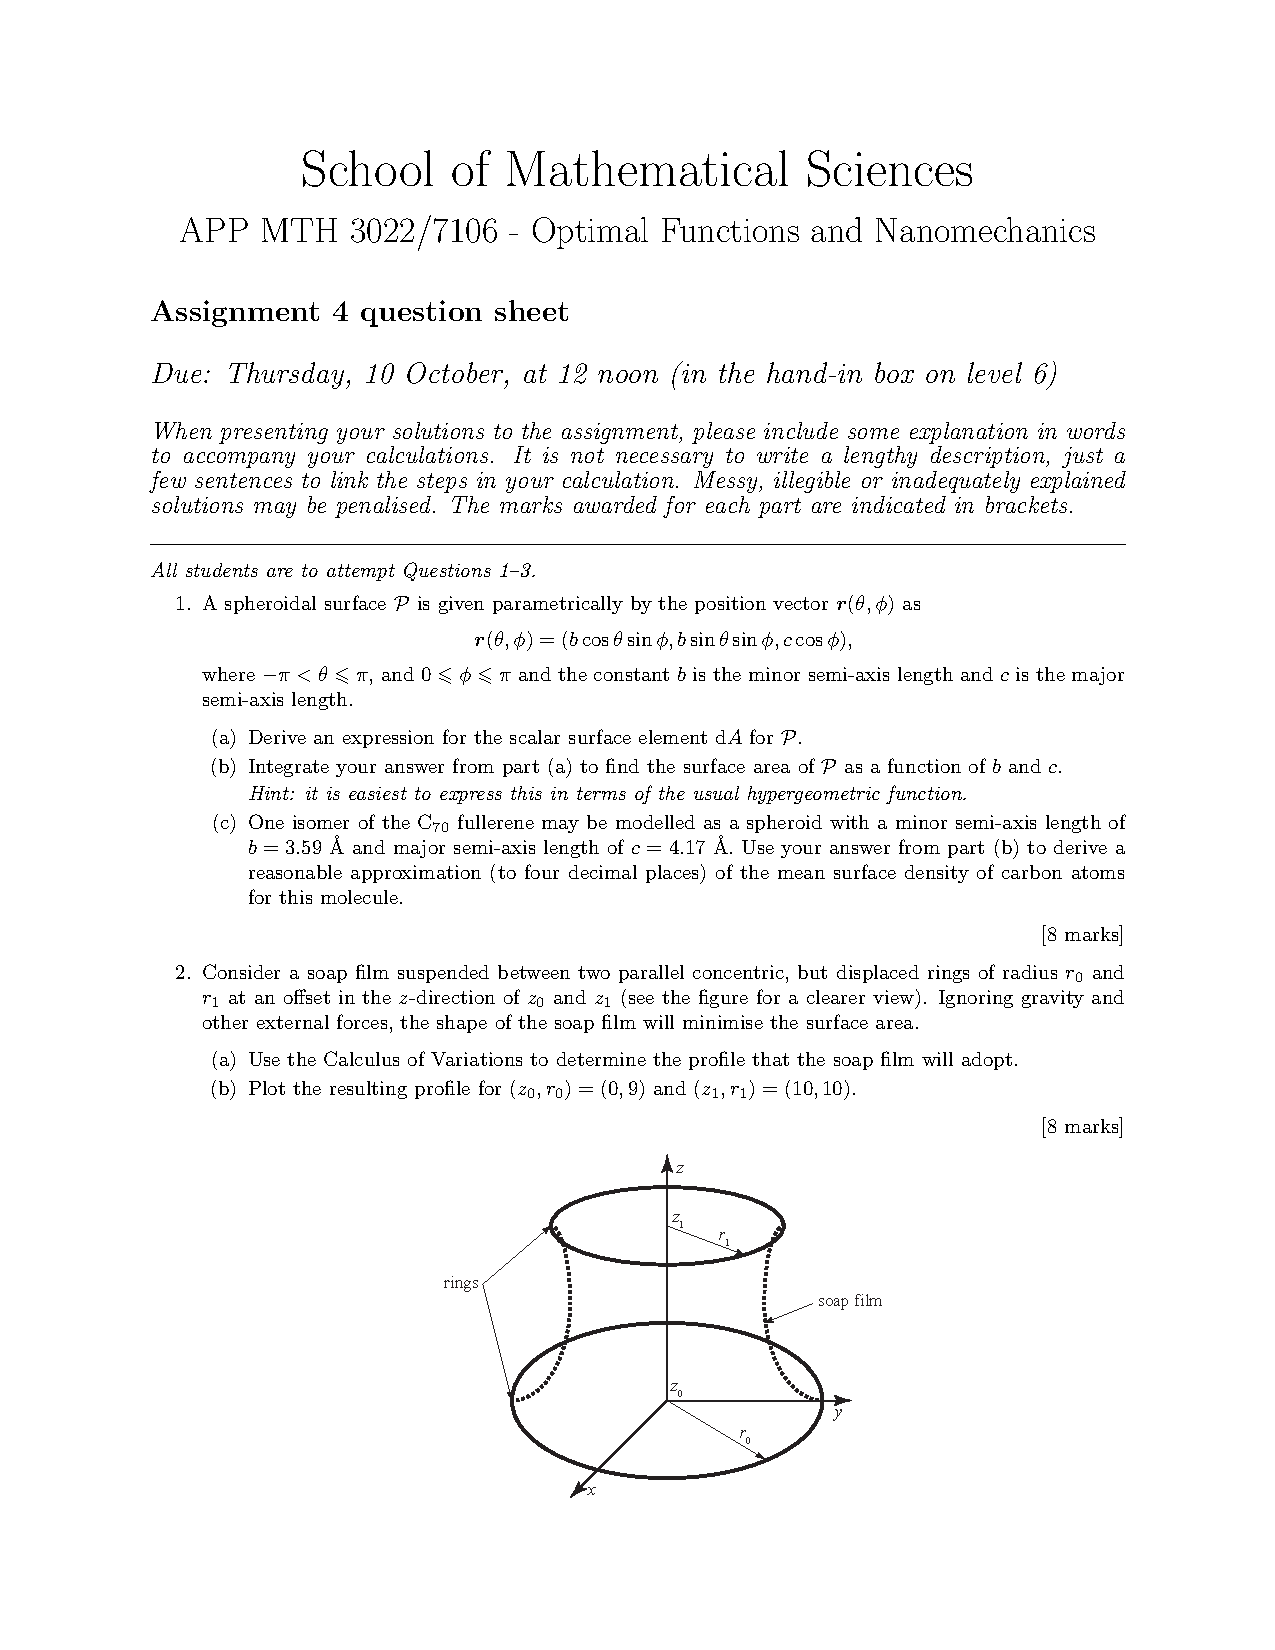
\includepdf[pages=1-]{assign4.pdf}

\end{document}